% anhang_f_staatsverschuldung.tex
\chapter{Anhang F: Staatsschulden und Generationengerechtigkeit}
\label{chap:anhang_f}

\section*{Einleitung}
Dieser Anhang analysiert den Zusammenhang zwischen deutschen Staatsschulden und der Entwicklung des Gemeinwohl-Index (GWI-D) unter besonderer Berücksichtigung der Generationengerechtigkeit.

\section{Entwicklung der Staatsverschuldung 1960–2023}

\begin{table}[ht]
    \centering
    \footnotesize
    \caption{Deutsche Staatsverschuldung: Historische Entwicklung}
    \label{tab:staatsverschuldung_entwicklung}
    \begin{tabular}{@{}lcccc@{}}
        \toprule
        \textbf{Epoche} & \textbf{Start} & \textbf{Ende} & \textbf{$\Delta$} & \textbf{Hauptursachen} \\
        & \textbf{(\% BIP)} & \textbf{(\% BIP)} & \textbf{(PP)} & \\
        \midrule
        1960–1973 & 18,2 & 16,8 & -1,4 & Wirtschaftswachstum \\
        1974–1982 & 16,8 & 41,5 & +24,7 & Ölkrise, Arbeitslosigkeit \\
        1983–1998 & 41,5 & 60,1 & +18,6 & Deutsche Einheit \\
        1999–2008 & 60,1 & 66,0 & +5,9 & Agenda-Reformen \\
        2009–2020 & 66,0 & 69,8 & +3,8 & Finanzkrise, Pandemie \\
        2021–2023 & 69,8 & 64,6 & -5,2 & Energiekrise, Inflation \\
        \bottomrule
    \end{tabular}
\end{table}

\begin{flushleft}
\scriptsize{\textit{Anmerkung: PP = Prozentpunkte. Positive $\Delta$ = Neuverschuldung, negative = Schuldenabbau.}}
\end{flushleft}

\begin{figure}[ht]
    \centering
    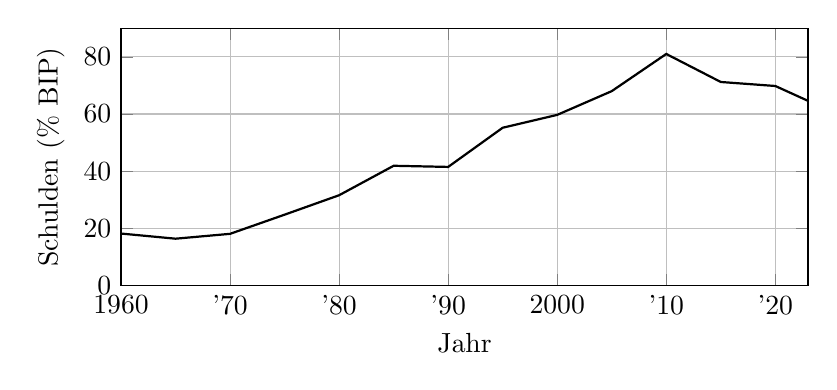
\begin{tikzpicture}
        \begin{axis}[
            width=0.85\textwidth,
            height=0.4\textwidth,
            xlabel={Jahr},
            ylabel={Schulden (\% BIP)},
            xmin=1960, xmax=2023,
            ymin=0, ymax=90,
            grid=both,
            xtick={1960,1970,1980,1990,2000,2010,2020},
            xticklabels={1960,'70,'80,'90,2000,'10,'20},
            ]
            \addplot[color=black, thick] coordinates {
                (1960,18.2) (1965,16.4) (1970,18.1) (1975,24.8)
                (1980,31.6) (1985,41.9) (1990,41.5) (1995,55.2)
                (2000,59.7) (2005,68.0) (2010,81.0) (2015,71.2)
                (2020,69.8) (2023,64.6)
            };
        \end{axis}
    \end{tikzpicture}
    \caption{Deutsche Staatsverschuldung 1960–2023}
    \label{fig:staatsverschuldung_verlauf}
\end{figure}

\section{Korrelationen mit GWI-D-Komponenten}

\begin{table}[ht]
    \centering
    \footnotesize
    \caption{Korrelation: Staatsverschuldung und GWI-D}
    \label{tab:korrelation_schulden_gwi}
    \begin{tabular}{@{}lcccc@{}}
        \toprule
        \textbf{Periode} & \textbf{W} & \textbf{G} & \textbf{Z} & \textbf{GWI-D} \\
        \midrule
        1960–2023 & 0,32 & 0,18 & 0,41 & 0,28 \\
        1960–1982 & -0,42 & 0,08 & -0,15 & -0,25 \\
        1983–2023 & 0,22 & 0,45 & 0,41 & 0,38 \\
        1999–2023 & 0,35 & 0,58 & 0,49 & 0,52 \\
        \bottomrule
    \end{tabular}
\end{table}

\begin{flushleft}
\scriptsize{\textit{Anmerkung: W = Wirtschaft, G = Gerechtigkeit, Z = Zukunft.}}
\end{flushleft}

\section{Generationenbilanz der Staatsverschuldung}

\begin{table}[ht]
    \centering
    \footnotesize
    \caption{Generationenkonten nach Geburtsjahrgängen}
    \label{tab:generationenkonten}
    \begin{tabular}{@{}lccc@{}}
        \toprule
        \textbf{Jahrgang} & \textbf{Nettobelastung} & \textbf{Anteil} & \textbf{G-Effekt} \\
        \midrule
        1940–1949 & -85.200 € & 18\% & +0,8 \\
        1950–1959 & -42.500 € & 22\% & +0,6 \\
        1960–1969 & +8.400 € & 24\% & -0,4 \\
        1970–1979 & +35.200 € & 18\% & -1,2 \\
        1980–1989 & +52.800 € & 12\% & -1,8 \\
        1990–1999 & +68.900 € & 6\% & -2,4 \\
        \bottomrule
    \end{tabular}
\end{table}

\begin{flushleft}
\scriptsize{\textit{Anmerkung: Werte in € pro Kopf, inflationsbereinigt 2023. G-Effekt = Einfluss auf Gerechtigkeitskomponente in GWI-D-Punkten.}}
\end{flushleft}

\section{Schuldentypologie und Gemeinwohleffekte}

\begin{table}[ht]
    \centering
    \footnotesize
    \caption{Gemeinwohleffekte verschiedener Schuldentypen}
    \label{tab:schuldentypen_wirkung}
    \begin{tabular}{@{}lp{3cm}ccc@{}}
        \toprule
        \textbf{Typ} & \textbf{Zweck} & \textbf{W} & \textbf{G} & \textbf{Nachhalt.} \\
        \midrule
        Investitionen & Bildung, Infrastruktur & ++ & + & Hoch \\
        Sozialinv. & Kinderbetreuung, Pflege & + & ++ & Mittel \\
        Konjunktur & Kurzarbeit, Soforthilfen & ++ & + & Niedrig \\
        Strukturerh. & Subventionen, Rettungen & + & - & Sehr niedrig \\
        Konsum & Laufende Ausgaben & - & - & Negativ \\
        \bottomrule
    \end{tabular}
\end{table}

\begin{flushleft}
\scriptsize{\textit{Anmerkung: ++ stark positiv, + positiv, - negativ.}}
\end{flushleft}

\section{Schuldenpolitik und Generationengerechtigkeit}

\begin{table}[ht]
    \centering
    \footnotesize
    \caption{Generationenübergreifende Transferwirkungen}
    \label{tab:transferwirkungen}
    \begin{tabular}{@{}lccc@{}}
        \toprule
        \textbf{Transfer} & \textbf{Finanzierung} & \textbf{Empfänger} & \textbf{GWI-D} \\
        \midrule
        Renten & Beitragszahler & Ältere & G: +0,5 \\
        Bildung & Steuern & Junge & Z: +1,2 \\
        Infrastruktur & Schulden & Alle & W: +0,8 \\
        Klimaschutz & Schulden & Zukunft & Z: +1,5 \\
        Krisenhilfen & Schulden & Gegenwart & W: +0,4 \\
        \bottomrule
    \end{tabular}
\end{table}

\section{Politische Steuerungsmechanismen}

\begin{table}[ht]
    \centering
    \footnotesize
    \caption{Vergleich nationaler Schuldenregeln}
    \label{tab:schuldenregeln_vergleich}
    \begin{tabular}{@{}lccc@{}}
        \toprule
        \textbf{Land} & \textbf{Regel} & \textbf{Flexibilität} & \textbf{Wirksamkeit} \\
        \midrule
        Deutschland & Schuldenbremse & Gering & Mittel \\
        Schweiz & Schuldenbremse & Mittel & Hoch \\
        USA & Keine Regel & Hoch & Niedrig \\
        Schweden & Überschussregel & Mittel & Hoch \\
        Japan & Keine Regel & Sehr hoch & Sehr niedrig \\
        \bottomrule
    \end{tabular}
\end{table}

\section{Alternativszenarien und Simulationen}

\begin{table}[ht]
    \centering
    \footnotesize
    \caption{Simulation alternativer Schuldenpfade}
    \label{tab:alternativszenarien}
    \begin{tabular}{@{}lccc@{}}
        \toprule
        \textbf{Szenario} & \textbf{Schulden 2040} & \textbf{GWI-D 2040} & \textbf{Generationen} \\
        \midrule
        Status quo & 75\% & 78,2 & Gering \\
        Investitionsoffensive & 85\% & 81,5 & Hoch \\
        Konsolidierungskurs & 55\% & 76,8 & Sehr gering \\
        \bottomrule
    \end{tabular}
\end{table}

\begin{flushleft}
\scriptsize{\textit{Anmerkung: Schulden in \% des BIP. Generationen = Bewertung der Generationengerechtigkeit.}}
\end{flushleft}

\section{Resümee: Schuldenpolitik als Gemeinwohlinstrument}

Die Analyse zeigt wichtige Erkenntnisse:

\begin{enumerate}
    \item \textbf{Schuldenqualität wichtiger als Höhe}: Investitionen in Bildung und Infrastruktur haben positive Gemeinwohleffekte.
    
    \item \textbf{Generationengerechtigkeit erfordert Balance}: Die heutige Schuldenpolitik bestimmt die Lastenverteilung zwischen Generationen.
    
    \item \textbf{Transparenz notwendig}: Klare Regeln und Generationenkonten helfen bei gemeinwohlorientierter Gestaltung.
    
    \item \textbf{Europäische Dimension}: Nationale Schuldenpolitik hat europäische Auswirkungen.
\end{enumerate}

\textbf{Abschließende Bewertung}: Die deutsche Schuldenpolitik hat gemischte Ergebnisse erzielt. Eine zukunftsorientierte Politik sollte stärker auf langfristige Gemeinwohleffekte und intergenerationelle Gerechtigkeit ausgerichtet sein.

\endinput